\documentclass{article}

\textwidth=6.5in
\textheight=8.5in
\voffset=-54pt
\oddsidemargin=0in
\evensidemargin=0in
\setlength{\parskip}{8pt}
\setlength{\parindent}{0pt}

\usepackage{amsmath, amssymb}
\usepackage{ifthen}

\usepackage[inline]{enumitem}
\setlist{topsep=0pt, parsep=8pt}

\usepackage[rgb,table]{xcolor}\convertcolorsUfalse
\usepackage{graphicx}

% change hyperref options
\PassOptionsToPackage{hyphens}{url}
\usepackage[bookmarks,colorlinks,linkcolor=black,citecolor=blue,pdfstartview=FitH,urlcolor=blue]{hyperref}
\hypersetup{pdfpagemode=UseNone}
\usepackage{bookmark}

\usepackage{graphicx}
\usepackage{multicol}
\usepackage{framed}
\usepackage{array}

\usepackage{icomma}

\usepackage{soul}
\usepackage[normalem]{ulem}

\usepackage{pgfplots}
\pgfplotsset{compat=1.18}  
\pgfplotscreateplotcyclelist{mycolor}{black, blue, red, green!70!black, magenta, purple, cyan, orange }  
\pgfplotsset{
  disabledatascaling,
  cycle list=tikzcolor, 
  axis lines=middle,
  every axis plot/.style={no marks, thick},
  every axis/.style={
    enlarge x limits=false,
    enlarge y limits=auto,
    xlabel style={at={(current axis.right of origin)},anchor=west},
    ylabel style={at={(current axis.above origin)},anchor=south},
    % extra x and y ticks for asymptotes
    extra x tick style={grid=major, grid style={dashed,black}},
    extra y tick style={grid=major, grid style={dashed,black}},
    /pgf/number format/1000 sep={},
  },    
  tick label style = {font=\footnotesize, fill=\currentbgcolor, inner sep=0pt},    
  xticklabel shift=1pt,    
  scaled ticks=false,
  scaled y ticks=false,
  unbounded coords=jump,
  samples=101,
  minor tick length=0,
  scatter/classes={
    open={mark=*,draw=black,fill=white, mark size=2, thin},
    closed={mark=*,draw=black,fill=black, mark size=2, thin}
  },
  width=3in,
}
\pgfplotsset{open/.style={only marks, mark=*, fill=white, thin, mark size=2}}
\pgfplotsset{closed/.style={only marks, mark=*, draw=black, fill=black,
    thin, mark size=2}}
\pgfplotsset{labeled/.style={nodes near coords, only marks, mark=*, draw=black, fill=black, thin, mark size=2, point meta=explicit symbolic}}

\usepackage{tikz}
\usetikzlibrary{
  matrix,%
  % enables the snake paths
  decorations.pathmorphing,%
  % enables bigger arrows
  decorations.markings,%
  decorations.pathreplacing,%
  decorations.text,%
  calc,%
  patterns,%
  shapes.geometric,%
  arrows,
  decorations.shapes,
  positioning,
  plotmarks,
  intersections
}
\tikzset{>=latex} % sets default arrow type in tikz
\tikzset{font=\normalsize}
\tikzset{mark size=1.5pt, mark options=thin}
\tikzset{pin distance=4pt,
  every pin edge/.style={<-, thin, shorten <= -2pt}}

\interfootnotelinepenalty=10000
\renewcommand{\thefootnote}{(\arabic{footnote})}

\usepackage{multirow, bigdelim}

% change to \usepackage[sols]{handout} to see solutions
\usepackage[
]{handout}

\newcommand\iscurrentenumi[1]{%
  \ifthenelse{\equal{#1}{\theenumi}}{}{#1}}
\setenumerate[1]{ref=\#\arabic*}
\setenumerate[2]{ref=\protect\iscurrentenumi{\theenumi}(\alph*)}
\newcommand\enumiiprefix[2]{%
  \ifthenelse{{\equal{#1}{\theenumi}}\AND{\equal{#2}{(\alph{enumii})}}}{}{}%
  \ifthenelse{{\equal{#1}{\theenumi}}\AND{\NOT{\equal{#2}{(\alph{enumii})}}}}{#2}{}%
  \ifthenelse{\equal{#1}{\theenumi}}{}{#1#2}%
}
\setenumerate[3]{ref=\protect\enumiiprefix{\theenumi}{(\alph{enumii})}\roman*}
% Make an environment that puts items in columns, first going across. 
\usepackage{tabto}
\newenvironment{enumeratecols}[2][]
{\NumTabs{#2}%
  \begin{enumerate*}[%before={\hspace{\dimexpr-\parindent-1pt}\tab},%
    itemjoin={\tab},#1]}%
  {\end{enumerate*}}

\newlength{\tipmargin}
\makeatletter

\newdimen\SOUL@dimen %new
\def\SOUL@ulunderline#1{{%
    \setbox\z@\hbox{#1}%
    % \dimen@=\wd\z@
    \SOUL@dimen=\wd\z@ %new
    \dimen@i=\SOUL@uloverlap
    \advance\SOUL@dimen2\dimen@i %\dimen@ exchanged too
    \rlap{%
      \null
      \kern-\dimen@i
      % \SOUL@ulcolor{\SOUL@ulleaders\hskip\dimen@}%
      \SOUL@ulcolor{\SOUL@ulleaders\hskip\SOUL@dimen}% new
    }%
    \unhcopy\z@
  }}

\renewenvironment{framed}{
  \setlength{\tipmargin}{\textwidth-\linewidth}
  \advance\@totalleftmargin-\tipmargin
  \def\FrameCommand{\hspace{\tipmargin}\fbox}%
  \advance\linewidth\tipmargin
  \MakeFramed {\advance\hsize-\width \FrameRestore}%
}
{\endMakeFramed}

\makeatother

\definecolor{purple}{rgb}{0.5,0,1.0}
\definecolor{hotpink}{rgb}{1, 0, 0.5}

\usepackage{fancyhdr}
\lhead{\textcolor{white}{This content is protected and may not be shared, uploaded, or distributed.}}
\rhead{}
\rfoot{\vspace*{\fill}\footnotesize\textcopyright{} \emph{Harvard Math Ma}}
\renewcommand{\headrulewidth}{0pt}
\pagestyle{fancy}
\begin{document}

\htitle{Maxima and Minima of Functions}

\begin{problemonly}
  \begin{framed}

You should be able to:
    \begin{itemize}[topsep=0pt,partopsep=0pt,parsep=8pt,itemsep=0pt]

    \item Explain the difference between a \emph{local minimum / maximum} and a \emph{global (or absolute) minimum / maximum}.

    \item Find the local extrema of a function by first finding \emph{critical points} and then using the First Derivative Test or Second Derivative Test.

    \item Explain why the First and Second Derivative Tests work.

    \end{itemize}
  \end{framed}
\end{problemonly}

\begin{enumerate}
\item 

  \note{This is just to set students up for thinking about the Second Derivative Test later.}

  \emph{Warm up.} Here's the graph of a function $f$.

  \begin{tikzpicture}[declare function={f(\x)=(33*\x)/2 - (25*\x^2)/2 + (19*\x^3)/6 - \x^4/4;}]
    \begin{axis}[hide y axis, ymin=0, height=2in, xtick={1, 3, 5.25}, xticklabels={$a$, $b$, $c$}]
      \addplot+[domain=0.5:6] {f(x)}; 
      \begin{scope}[dashed, gray, thin]
        \draw (1, 0) -- (1, {f(1)}); %
        \draw (3, 0) -- (3, {f(3)}); %
        \draw (5.25, 0) -- (5.25, {f(5.25)}); % 
      \end{scope}
    \end{axis}
  \end{tikzpicture}

  \begin{enumerate}
  \item Based on the graph, are each of the following positive, negative, or zero?

    \probonly{\begin{enumeratecols}{3}}\solonly{\begin{enumerate}}
      \item
        \begin{problem}
          $f'(a)$
        \end{problem}

        \begin{solution}
          0
        \end{solution}

      \item
        \begin{problem}
          $f'(b)$
        \end{problem}

        \begin{solution}
          0
        \end{solution}

      \item
        \begin{problem}
          $f'(c)$
        \end{problem}

        \begin{solution}
          Positive
        \end{solution}

      \solonly{\end{enumerate}}\probonly{\end{enumeratecols}}

  \pspace{\vfill}

  \item Based on the graph, are each of the following positive or negative?

    \probonly{\begin{enumeratecols}{3}}\solonly{\begin{enumerate}}
      \item
        \begin{problem}
          $f''(a)$
        \end{problem}

        \begin{solution}
          Negative
        \end{solution}

      \item
        \begin{problem}
          $f''(b)$
        \end{problem}

        \begin{solution}
          Positive
        \end{solution}

      \item
        \begin{problem}
          $f''(c)$
        \end{problem}

        \begin{solution}
          Negative
        \end{solution}

      \solonly{\end{enumerate}}\probonly{\end{enumeratecols}}

  \pspace{\nstretch{2}}
  \end{enumerate}

\end{enumerate}
\note{At this point, I'll give some motivation of why we might want to optimize functions. After that, I'll probably talk about how the derivative is our main tool, but it only tells us about local behavior; so, even though we're primarily interested in global extrema for applications, a reasonably strategy is to first find local extrema.}

\begin{enumerate}[resume]
\item  % based on Peter Garfield's worksheet 

  \note{Here, I just want students to think about where local and global extrema can occur in a variety of pictures.}

  \begin{enumerate}
  \item \label{identify-local-extrema} 
    Intuitively, a \uline{local maximum} of $f$ is a point on the graph of $f$ that's at least as high as all nearby points. More precisely, $f$ has a local maximum at $c$ if $f(c) \geq f(x)$ for all $x$ near $c$. Mark the local maxima and local minima on the graphs below.    

    \begin{tikzpicture}[declare function={f(\x)=abs((\x+0.5)^2-1)+.25;}]
      \begin{axis}[width=2.25in, xtick={-1.8, 1.8}, xticklabels={$a$, $b$}, ytick=\empty]
        \addplot+[domain=-2:0.75] {f(x)};
        \addplot+[sharp plot] coordinates {(0.75, {f(0.75)}) (2, {f(0.75) + 0.25})}; 
        \solonly{%
          \addplot+[closed, red] coordinates { (-1.5, {f(-1.5)}) };%
          \addplot+[closed, red] coordinates { (0.5, {f(-1.5)}) };%
          \draw (-0.5, {f(-1.5)}) node[red, fill=white, inner sep=1pt] {local mins};%
          \addplot+[closed, blue] coordinates {(-0.5, {f(-0.5)}) } node[anchor=south west, fill=white]{local max}; %
        }
      \end{axis}
    \end{tikzpicture}
    \qquad
    \begin{tikzpicture}[declare function={f(\x)=\x^2*(\x-1.5)*(\x+1.75)/3-0.5;}]
      \begin{axis}[width=2.25in, clip=false, xtick={-1.8, 1.8}, xticklabels={$a$, $b$}, ytick=\empty]
        \addplot[domain=-2:2] {f(x)}; %
        \solonly{%
          \addplot+[closed, red] coordinates { (-1.24322, {f(-1.24322)}) } node[below]{local min};%
          \addplot+[closed, red] coordinates { (1.05572, {f(1.05572)}) } node[below]{local min};%
          \addplot+[closed, blue] coordinates {(0, {f(0)}) } node[above, fill=white, inner sep=1pt, yshift=1pt]{local max}; %
        }
      \end{axis}
    \end{tikzpicture}
    \qquad
    \begin{tikzpicture}
      \begin{axis}[width=2.25in, restrict y to domain=-4:4, ymin=-3.5, ymax=3.5, extra x ticks={-1, 1}, xtick={-1.8, 1.8}, xticklabels={$a$, $b$}, extra x tick labels={}, ytick=\empty]
        \addplot [domain=-2:2] {.3/((x+1)*(x-1))}; %
        \addplot [domain=-.9:.9] {.3/((x+1)*(x-1))};%
        \solonly{%
          \addplot+[closed, blue] coordinates {(0, -0.3) } node[above, fill=white]{local max}; %
        }
      \end{axis}
    \end{tikzpicture}    

  \item

    \note{In the first picture, the global minimum is achieved in 2 places. I want to make clear that there can only be one global minimum value, but it can be achieved in multiple places.}

    \begin{problem}[\vfill]
      We say that a function $f$ has a \uline{global maximum} (also known as an \uline{absolute maximum}) at $c$ if $f(c)$ is the highest value of $f$ anywhere in the domain; more precisely, $f$ has a global maximum at $c$ if $f(c) \geq f(x)$ for all $x$ in the domain.

      For each graph in \ref{identify-local-extrema}, does $f$ have a global minimum and a global maximum on $[a, b]$? If so, mark where $f$ achieves its global maximum and global minimum values. 
    \end{problem}

    \solonly{
        \begin{tikzpicture}[declare function={f(\x)=abs((\x+0.5)^2-1)+.25;}]
      \begin{axis}[width=2.25in, xtick={-1.8, 1.8}, xticklabels={$a$, $b$}, ytick=\empty]
        \addplot+[domain=-2:0.75] {f(x)};
        \addplot+[sharp plot] coordinates {(0.75, {f(0.75)}) (2, {f(0.75) + 0.25})}; 
        \solonly{%
          \addplot+[closed, red] coordinates { (-1.5, {f(-1.5)}) };%
          \addplot+[closed, red] coordinates { (0.5, {f(-1.5)}) };%
          \draw (-0.5, {f(-1.5)}) node[red, fill=white, inner sep=1pt] {global mins};%
          \addplot+[closed, blue] coordinates {(-0.5, {f(-0.5)}) } node[anchor=south west, fill=white]{global max}; %
        }
      \end{axis}
    \end{tikzpicture}
    \qquad
    \begin{tikzpicture}[declare function={f(\x)=\x^2*(\x-1.5)*(\x+1.75)/3-0.5;}]
      \begin{axis}[width=2.25in, clip=false, xtick={-1.8, 1.8}, xticklabels={$a$, $b$}, ytick=\empty]
        \addplot[domain=-2:2] {f(x)}; %
        \solonly{%
          \addplot+[closed, red] coordinates { (-1.24322, {f(-1.24322)}) } node[below]{global min};%
          \addplot+[closed, blue] coordinates {(1.8, {f(1.8)}) } node[above, fill=white, inner sep=1pt, yshift=1pt]{global max}; %
        }
      \end{axis}
    \end{tikzpicture}
    \qquad
    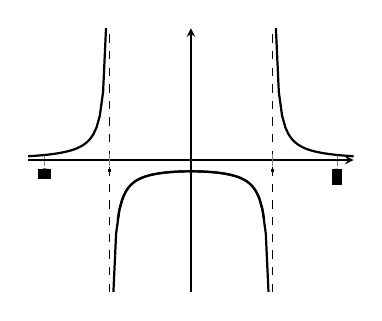
\begin{tikzpicture}
      \begin{axis}[width=2.25in, restrict y to domain=-4:4, ymin=-3.5, ymax=3.5, extra x ticks={-1, 1}, xtick={-1.8, 1.8}, xticklabels={$a$, $b$}, extra x tick labels={}, ytick=\empty]
        \addplot [domain=-2:2] {.3/((x+1)*(x-1))}; %
        \addplot [domain=-.9:.9] {.3/((x+1)*(x-1))};%
      \end{axis}
    \end{tikzpicture}   
    }

  \item

    \note{It can be confusing to students that a graph like the second one above doesn't have a global maximum on $(a, b)$; make sure they understand that when we talk about a global maximum, we're talking about a point \emph{on the graph} that's at least as high as all other points on the graph.}

    \begin{problem}[\vfill]
      For each of the above graphs, does $f(x)$ have a global minimum and a global maximum on $(a, b)$? If so, where?
    \end{problem}

    \solonly{
    \begin{tikzpicture}[declare function={f(\x)=abs((\x+0.5)^2-1)+.25;}]
      \begin{axis}[width=2.25in, xtick={-1.8, 1.8}, xticklabels={$a$, $b$}, ytick=\empty]
        \addplot+[domain=-2:0.75] {f(x)};
        \addplot+[sharp plot] coordinates {(0.75, {f(0.75)}) (2, {f(0.75) + 0.25})}; 
        \solonly{%
          \addplot+[closed, red] coordinates { (-1.5, {f(-1.5)}) };%
          \addplot+[closed, red] coordinates { (0.5, {f(-1.5)}) };%
          \draw (-0.5, {f(-1.5)}) node[red, fill=white, inner sep=1pt] {global mins};%
          \addplot+[closed, blue] coordinates {(-0.5, {f(-0.5)}) } node[anchor=south west, fill=white]{global max}; %
        }
      \end{axis}
    \end{tikzpicture}
    \qquad
    \begin{tikzpicture}[declare function={f(\x)=\x^2*(\x-1.5)*(\x+1.75)/3-0.5;}]
      \begin{axis}[width=2.25in, clip=false, xtick={-1.8, 1.8}, xticklabels={$a$, $b$}, ytick=\empty]
        \addplot[domain=-2:2] {f(x)}; %
        \solonly{%
          \addplot+[closed, red] coordinates { (-1.24322, {f(-1.24322)}) } node[below]{global min};%
        }
      \end{axis}
    \end{tikzpicture}
    \qquad
    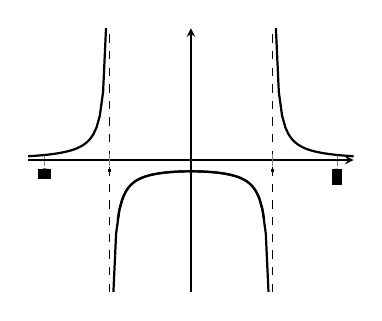
\begin{tikzpicture}
      \begin{axis}[width=2.25in, restrict y to domain=-4:4, ymin=-3.5, ymax=3.5, extra x ticks={-1, 1}, xtick={-1.8, 1.8}, xticklabels={$a$, $b$}, extra x tick labels={}, ytick=\empty]
        \addplot [domain=-2:2] {.3/((x+1)*(x-1))}; %
        \addplot [domain=-.9:.9] {.3/((x+1)*(x-1))};%
      \end{axis}
    \end{tikzpicture}   
    }

  \end{enumerate}

\item  % Peter Garfield

  \begin{enumerate}

  \item

    \note{Here, the goal is to get students to come up with the definition of critical points. (I'll have them look back at the examples in \ref{identify-local-extrema}.)}

    \begin{problem}[\stretch{0.75}]
      Often, our goal is to find the global minimum or maximum (if it exists) of a function on a given interval. A good starting point is to first find the local extrema (``local extremum'' is a shorthand way of saying ``local minimum or local maximum'').

      What can you say about $f'(c)$ at a value $c$ where $f$ has a local
      extremum?
    \end{problem}

    \begin{solution}
      $f'(c)$ is 0 or undefined.
    \end{solution}

  \end{enumerate}

  \begin{framed}
    \textbf{Definition.} A \uline{critical point} of $f$ is a number $c$ in the domain of $f$ such that\probonly{\ldots} \solonly{$f'(c)$ is zero or undefined.}

    \pspace{0.25in}

    \emph{Note:} The Gottlieb textbook has a slightly different definition; it also considers endpoints of the domain to be critical points, while we don't. 
  \end{framed}

  \pspace{\newpage}

  \begin{enumerate}[resume]
  \item

    \note{Here, I'll have them look back at \ref{identify-local-extrema} to see that not every critical point is a local extremum. If I remember, I will also ask if they can draw an example where $f'(c) = 0$ but $c$ isn't a local extremum (like $f(x) = x^3$ at $0$).}

    \begin{problem}[\stretch{0.5}]
      Is every critical point a local minimum or local maximum?  
    \end{problem}

    \begin{solution}
      No! For example, in \ref{identify-local-extrema}, here's a critical point that is neither a local minimum nor a local maximum:
      \begin{center}
        \begin{tikzpicture}[declare function={f(\x)=abs((\x+0.5)^2-1)+.25;}]
          \begin{axis}[width=2.25in, xtick={-1.8, 1.8}, xticklabels={$a$, $b$}, ytick=\empty]
            \addplot+[domain=-2:0.75] {f(x)}; %
            \addplot+[sharp plot] coordinates {(0.75, {f(0.75)}) (2, {f(0.75) + 0.25})}; % 
            \addplot+[closed, hotpink] coordinates { (0.75, {f(0.75)}) }; 
          \end{axis}
        \end{tikzpicture}
      \end{center}
    \end{solution}

  \item

    \note{As the pictures in \ref{identify-local-extrema} illustrate, we need to look at ends of the domain and places where $f$ is discontinuous.}

    \begin{problem}[\stretch{0.5}]
      Besides looking at local extrema, where else should we look to see
      if a function has global extrema on a given interval?
    \end{problem}

    \begin{solution}
      Ends of the domain and places where $f$ is discontinuous. 
    \end{solution}

  \end{enumerate}

\item   \label{analyze-cubic-1}

  In this problem, we'll look at the function $f(x) = x^3 + 3x^2 + 1$.
  \begin{enumerate}
  \item
    \begin{problem}[\stretch{0.75}]
      Find all critical points of $f$.
    \end{problem}

    \begin{solution}
      $f'(x) = 3x^2 + 6x = 3 (x^2 + 2x) = 3 x (x + 2)$, so $f'(x) = 0$ at $x = \boxed{-2, 0}$. (There are no points where $f'$ is undefined.)
    \end{solution}

  \item
    \begin{problem}[\vfill]
      Make a sign chart for $f'$, and use this to decide whether each of
      the critical points you found is a local minimum, a local maximum,
      or neither.
    \end{problem}

    \probonly{\emph{What you just did is called the \textbf{First
          Derivative Test} to decide whether a critical point is a local
        minimum, a local maximum, or neither.}}

    \begin{solution}
      \begin{center}
        \begin{tikzpicture}
          \begin{axis}[axis y line=none, x axis line style={-}, xtick={-2, 0}, ymin=-2, height=1in, width=3in, clip=false]
            \addplot+[domain=-6:2, very thin]{0};
            \draw (axis cs: -6, -1.5) node[right] {sign of $f'$};
            \draw (axis cs: -3, -1.5) node{$+$};
            \draw (axis cs: -1, -1.5) node{$-$};
            \draw (axis cs: 1, -1.5) node{$+$};
          \end{axis}
        \end{tikzpicture}
      \end{center}
      So, there is a local maximum at $x = -2$ and a local minimum at $x = 0$.
    \end{solution}

  \end{enumerate}

  \pspace{\newpage}

\item  

  \note{The goal here is for students to figure out most of the Second Derivative Test. This isn't that natural for them, so be prepared to guide them.}

  There's another way to decide whether a critical point is a local min, local max, or neither. That's what we'll look at in this problem!

  Let $f(x) = x^4 - 8x^2 + 16$.
  \begin{enumerate}
  \item
    \begin{problem}[\vfill]
      Find all critical points of $f$. 
    \end{problem}

    \begin{solution} 
      To find the critical points, we need to know when the derivative equals 0. 
        $$f'(x) = 4x^3-16x$$
        $$f'(x) =4x(x^2-4)=0$$ 
        So the critical points are
        $$x=-2,\text{ } 0, \text{and } 2$$
    \end{solution} 

  \item
    \begin{problem}[\vfill]
      For each critical point $c$ of $f$, find the sign of $f''(c)$.
      What does this tell you about the critical point $c$?
    \end{problem}

    \begin{solution} 
       $f''(x) = 12x^2-16$
      \begin{multicols}{3}    
          \begin{tabular} {c | c} 
            $x$ & $f''(x)$ \\ 
            \hline \\
            0 & -16\\
            & \\
            2 & 32\\ 
            & \\ 
            -2 & 32 
          \end{tabular} 

          Note that a critical point on a concave up portion of the graph is a local min and a critical point on a concave down portion of the graph is a local max.  

        \vspace{ .2 in } 

        \hfill \begin{tikzpicture} [xscale =.25, yscale =.25]
          \begin{axis}[hide axis]

            \addplot+[domain=-2:2] [ultra thick,green] {x^2};

          \end{axis}
        \end{tikzpicture} 
        \begin{tikzpicture} [xscale =.25, yscale =.25]
          \begin{axis}[hide axis]

            \addplot+[domain=-2:2] [ultra thick,blue] {-x^2};
          \end{axis}
        \end{tikzpicture} 
      \end{multicols} 

      We know that there is a local max at $x=0$, and there are local minima at $x=\pm 2$.

    \end{solution}

  \item
    \begin{problem}[\stretch{0.2}]
      On what intervals is $f$ increasing?  On what intervals is it
      decreasing?  (How little additional work can you do to answer this
      question?) 
    \end{problem}

    \begin{solution}
      We know that $f$ has $3$ critical points and we've already classified them.
      From our classifications, we can deduce that $f$ decreases on $(-\infty, -2)$,
      increases on $(-2, 0)$, decreases on $(0, 2)$, and increases on $(2, \infty)$. 
    \end{solution}

  \end{enumerate}

\item  

  \note{This demonstrates that the Second Derivative Test must be inconclusive when the second derivative is 0.}

  Let $f(x) = x^3$ and $g(x) = x^4$.
  \begin{enumerate}
  \item

    \note{$x^4$ isn't a function they're so familiar with, but it's pretty easy to see that it's even and increasing on $(0, \infty)$.}

    \begin{problem}[\vfill\newpage]
      Sketch graphs of $f(x)$ and $g(x)$.
    \end{problem}

    \begin{solution}
      $g(x)$ is sketched in blue. $f(x)$ is sketched in red. 

      \hfill 
      \begin{tikzpicture} [xscale =.6, yscale =.6]
        \begin{axis}[]

          \addplot+[domain=-2:2] [blue] {x^4};

        \end{axis}
      \end{tikzpicture}  \hfill \begin{tikzpicture} [xscale =.6, yscale =.6]
        \begin{axis}[]

          \addplot+[domain=-2:2] [red] {x^3};

        \end{axis}
      \end{tikzpicture} \hfill b

    \end{solution}

  \item
    \begin{problem}[0.75in]
      What is $f'(0)$?  $f''(0)$? 
    \end{problem}

    \begin{solution} 
       $f'(x) = 3x^2$ and $f''(x) = 6x$. So  $f'(0)=f''(0)=0$.
    \end{solution} 

  \item
    \begin{problem}[0.75in]
      What is $g'(0)$? $g''(0)$?
    \end{problem}

    \begin{solution} 
       $g'(x) = 4x^3$ and $g''(x) = 12x^2$. So  $g'(0)=g''(0)=0$.

        Notice that both $f$ and $g$ have second derivative 0 at the critical point 0, but $f$ has a local min at $x = 0$ and $g$ has neither a local min nor a local max at $x = 0$. So, having second derivative 0 at a critical point doesn't tell us what type of critical point that is.
    \end{solution} 

  \end{enumerate}

\end{enumerate}
\begin{framed}
  \textbf{Second Derivative Test.} Suppose $f'(c) = 0$.  What can you
  conclude if you have the following additional information about
  $f''(c)$?
  \begin{itemize}
  \item $f''(c) > 0$.

    \begin{solution}
      $c$ is a local min.
    \end{solution} 

  \item $f''(c) < 0$.

    \begin{solution}
      $c$ is a local max.
    \end{solution} 

  \item $f''(c) = 0$.

    \begin{solution}
      No information.
    \end{solution}

  \end{itemize}  
\end{framed}

\note{Going over the Second Derivative Test is the last thing we really need to do, but I hope we'll have time to do one more problem.}

\begin{enumerate}[resume]
\item 

  \note{This includes a critical point where $f'$ is undefined (and therefore the Second Derivative Test is useless).}

  \begin{problem}[\vfill]    
    Let $f(x) = 3x^{2/3} - x$. Find all critical points of $f$, and classify each as a local minimum, local maximum, or neither. (Do you find the First Derivative Test or Second Derivative Test more useful here?)
  \end{problem}

  \begin{solution}
    To find the critical points, we need to know where $f'(x)$ is zero or undefined. Using
    the power rule, $f'(x) = 2x^{-1/3}-1$, which is undefined when $x=0$. We can solve
    $f'(x)=0$ for $x$:
    \begin{align*}
      2x^{-1/3} -1 &= 0 \\
      \frac{2}{x^{1/3}} &= 1 \\
      2 &= x^{1/3} \\
      x &= 8.
    \end{align*}
    The critical points are $x=0$ and $x=8$. 
    To use the First Derivative Test, we can put these values on a sign chart.
    \begin{center}
        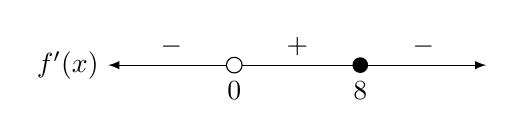
\begin{tikzpicture}[scale=0.8]
          \draw[<->] (-3,0) -- (3, 0);
          \node[left] at (-3,0) {$f'(x)$};
          \draw[shift={(-1,0)},color=black] (0pt,3pt) -- (0pt,-3pt) node[below] {$0$};
          \draw[shift={(1,0)},color=black] (0pt,3pt) -- (0pt,-3pt) node[below] {$8$};
          \node[circle, fill=black, inner sep=2pt] at (1,0) {};
          \node[circle, draw=black, fill=white, inner sep=2pt] at (-1,0) {};
          \node[above] at (-2,0) {$-$};
          \node[above] at (0,0) {$+$};
          \node[above] at (2,0) {$-$};
        \end{tikzpicture}
      \end{center}
     Since $f'$ changes from negative to positive at $x=0$, there a a local minimum at $x=0$.
     Since $f'$ changes from positive to negative at $x=8$, there is a local maximum at $x=8$.

     The Second Derivative Test would not have worked to classify the critical point
     at $x=0$, because $f'(0)$ and $f''(0)$ are undefined. 
     We have to use the First Derivative Test
     in this case.
  \end{solution}

\item 
  \begin{problem}[\nstretch{0.5}]
    What are advantages and disadvantages of the Second Derivative Test
    vs.\ the First Derivative Test?
  \end{problem}

  \begin{solution}
    The main advantage of the Second Derivative Test is that we only need to determine
    the sign of the
    the second derivative at the critical point, unlike the First Derivative Test,
    where we need to determine the sign of the first derivative on either side of
    the critical point.

    The disadvantages of the Second Derivative Test are that we need to calculate the
    second derivative in addition to the first derivative,
    and that the Second Derivative Test is sometimes
    inconclusive, e.g. at critical points where the first derivative is undefined, 
    or when the second derivative is zero.
  \end{solution}

\item  

  \note{This is also on the next worksheet; I've just put it here in case we have extra time.}

  \label{critical-points-reasoning-set2}

  Suppose you've made the following sign chart for the derivative of a
  function $f(x)$.  The function $f(x)$ is continuous and differentiable
  on $(-\infty, \infty)$.
  \begin{center}
    \begin{tikzpicture}
      \begin{axis}[axis y line=none, x axis line style={-}, xtick={0, 3, 5}, ymin=-2, height=1in, width=3.5in, clip=false]
        \addplot+[domain=-6:7.5, very thin]{0};
        \draw (-6, -1.5) node[right] {sign of $f'$};
        \draw (-1.25, -1.5) node{$+$};%
        \draw (1.5, -1.5) node{$-$};%
        \draw (4, -1.5) node{$+$};%
        \draw (6.25, -1.5) node{$-$};%
      \end{axis}
    \end{tikzpicture}    
  \end{center}

  \begin{enumerate}
  \item

    \note{It's worthwhile to ask students how they'd decide where the global maximum was is if they had the formula for $f$ (to get them to think of evaluating $f(0)$ and $f(5)$ as a simple way).}

    \begin{problem}[\vfill]
      Does $f$ have a global maximum on $(-\infty, \infty)$? (Definitely yes, definitely no, or maybe?) If so, where could it be?
    \end{problem}

    \begin{solution}
      Yes, $f$ must have a global maximum at either $x = 0$ or $x = 5$.
    \end{solution}

  \item

    \note{Students may forget about the possibility of horizontal asymptotes here.}

    \begin{problem}[\vfill]
      Does $f(x)$ have a global minimum on $(-\infty, \infty)$? If so, where could it be?
    \end{problem}

    \begin{solution}
      There is not enough information to be sure. For example, it's possible that $\displaystyle \lim_{x \to \infty} f(x) = - \infty$, in which case $f$ certainly would not have a global minimum. However, it's also possible that $\displaystyle \lim_{x \to \infty} f(x)$ and $\displaystyle \lim_{x \to -\infty} f(x)$ both exist and that $x = 3$ is a global minimum point. Both possibilities are illustrated below:
      \begin{center}
        \begin{tikzpicture}
          \begin{axis}[xtick={3, 5}, ytick=\empty, enlargelimits=false,
            width=3in, ymax=600, clip=false] 
            \addplot+[domain=-2:7.5, samples=151]{500 - 90*x^2 + 32*x^3 -
              3*x^4}; 
          \end{axis}
        \end{tikzpicture}
        \hspace{0.5in}
        \begin{tikzpicture}
          \begin{axis}[xtick={3, 5}, ytick=\empty, enlargelimits=false,
            width=3in, ymin=0, extra y ticks={1}, extra y tick labels={},
            clip=false] 
            \addplot+[domain=-4:8]{2.718281828459045^(((-4.274856759437754 + x)*(-1.058476573895579 + x))/(1. + (-3.0676437038635322 + x)^2)^2)};
          \end{axis}
        \end{tikzpicture}
      \end{center}
    \end{solution}

  \item
    \begin{problem}[\vfill]
      Does $f$ have a global maximum on $[-2, 10]$?  If so, where could
      it be?
    \end{problem}

    \begin{solution}
      Yes, $f$ must have a global maximum on $[-2, 10]$; it could be at $x = 0$ or $x = 5$.
    \end{solution}

  \item
    \begin{problem}[\vfill]
      Does $f$ have a global minimum on $[-2, 10]$? If so, where could it be?
    \end{problem}

    \begin{solution}
      Yes, $f$ must have a global minimum on $[-2, 10]$; it could be at $x = -2$, $x = 3$, or $x = 10$.
    \end{solution}

  \end{enumerate}

\item  \label{analyze-cubic-1-followup}

  Let's look again at $f(x) = x^3 + 3x^2 + 1$ from \ref{analyze-cubic-1}.
  \begin{enumerate}
  \item

    \note{From the sign chart, the global maximum must occur either at $x = -4$ and $x = 0$. As we get more into optimization, students often get confused about how to test which is the right one, so try to get them to think about what information they need. (If they're just trying to decide which of these two produces the higher point, just plug into the function.)}

    \begin{problem}[\vfill]
      Does $f$ have a global maximum on $[-4, 0]$?  If so, where?  How
      about a global minimum?
    \end{problem}

    \begin{solution}
      In \ref{analyze-cubic-1}, we found the following sign chart for
      $f'$:
      \begin{center}
        \begin{tikzpicture}
          \begin{axis}[axis y line=none, x axis line style={-}, xtick={-2., 0.}, xticklabels={$-2$, $0$}, ymin=-2, ymax=2, height=1.25in, width=3in]
            \addplot+[domain=-6.:2., very thin]{0};
            \draw (axis cs: -6., -1.5) node[right] {sign of $f'$};
            \draw (axis cs: -6., 1) node[right] {$f$};
            \draw (axis cs: -3., -1.5) node{$+$};
            \draw[->, xshift=2pt] (axis cs: -5.46667, 0.5) -- (axis cs: -2.26667, 1.5);
            \draw (axis cs: -1., -1.5) node{$-$};
            \draw[->, xshift=2pt] (axis cs: -1.73333, 1.5) -- (axis cs: -0.266667, 0.5);
            \draw (axis cs: 1., -1.5) node{$+$};
            \draw[->, xshift=2pt] (axis cs: 0.266667, 0.5) -- (axis cs: 1.73333, 1.5);
            \draw[->, xshift=2pt] (axis cs: -2.26667, 1.5) -- (axis cs: -1.73333, 1.5);
            \draw[->, xshift=2pt] (axis cs: -0.266667, 0.5) -- (axis cs: 0.266667, 0.5);
          \end{axis}
        \end{tikzpicture}
      \end{center}
      So, on $[-4, 0]$, $f$ must have an \fbox{global maximum at $x =
        -2$}.  Also, it has a global minimum at either $x = -4$ or $x =
      0$, but the sign chart doesn't tell us which.  To decide, we simply
      need to know whether $f(-4)$ or $f(0)$ is lower, so we evaluate
      both:
      \begin{align*}
        f(-4) &= -15 \\
        f(0) &= 1
      \end{align*}
      So, on $[-4, 0]$, $f$ has an \fbox{global minimum at $x = -4$}. 
    \end{solution}

  \item
    \begin{problem}[\vfill]
      Does $f$ have a global maximum on $[-4, 2]$?  If so, where?  How
      about a global minimum?
    \end{problem}

    \begin{solution}
      The sign chart shows us that $f$ has a global maximum on $[-4,
      2]$ at either $-2$ or $2$; to decide which, we see which has the
      higher value of $f$:
      \begin{align*}
        f(-2) &= 5 \\
        f(2) &= 21
      \end{align*}
      So, the \fbox{global maximum is at $x = 2$}.  We already found
      that the global minimum of $f$ on $[-4, 0]$ was at $x = -4$; since
      $f$ is increasing on $(0, 2)$, \fbox{$x = -4$ must also be where its
        minimum on $[-4, 2]$ is}.
    \end{solution}

  \item

    \note{It can be tricky for students to figure out that they need to
      compare $f(-2)$ with $\displaystyle \lim_{x \to 3^-} f(x)$ to see
      whether $f$ has a global maximum.}

    \begin{problem}[\vfill]
      Does $f$ have a global maximum on $(-3, 3)$?  If so, where?  How
      about a global minimum?
    \end{problem}

    \begin{solution}
      From the sign chart alone, it's not obvious.  It's possible that $f$
      has a global maximum at $x = -2$, but it's also possible that $f$
      gets higher than this as $x$ approaches $3$.  To test, let's compare
      $f(-2)$ with $\displaystyle \lim_{x \to 3^-} f(x)$:
      \begin{align*}
        f(-2) &= 5 \\
        \lim_{x \to 3^-} f(x) &= 55
      \end{align*}
      So, $f$ has \fbox{no global maximum on $(-3, 3)$}.

      Similarly, to decide whether $f$ has a global minimum on $(-3,
      3)$, we should compare $f(0)$ and $\displaystyle \lim_{x \to -3^+}
      f(x)$:
      \begin{align*}
        f(0) &= 1 \\
        \lim_{x \to -3^+} f(x) &= 1 
      \end{align*}
      Let's think carefully about what this means.  Since $f$ is
      increasing for $x < -2$, this means that, as $x$ approaches $-3$
      from the right, its values approach 1 but are always greater than
      1.  Therefore, $f(0) = 1$ is the lowest value $f$ ever achieves on
      $(-3, 3)$, so $f$ has an \fbox{global minimum at $x = 0$}. 
    \end{solution}

  \end{enumerate}

\item 
  \begin{problem}[\vfill]
    Does $f(x) = x - 2 + \frac{1}{x}$ have a global minimum on $(0, \infty)$? If so, where? Does $f$ have a global maximum on $(0, \infty)$? If so, where?
  \end{problem}

  \begin{solution}
    Let's start by making a sign chart for $f'(x) = 1 - x^{-2} = 1 - \frac{1}{x^2}$. On $(0, \infty)$, $f'$ is never undefined, and it's 0 when $x = 1$. We can test, for example, the following values:
    \begin{align*}
      f' \left( \frac{1}{2} \right) &= 1 - 2^2 < 0 \\
      f' (2) &= 1 - \frac{1}{4} > 0 
    \end{align*}
    This gives us the following sign chart:
    \begin{center}
      \begin{tikzpicture}
        \begin{axis}[axis y line=none, x axis line style={-}, xtick={1}, ymin=-2, ymax=2, height=1.25in, width=3in]
          \addplot+[domain=-1.5:3., very thin]{0};
          \draw (axis cs: -1.5, -1.5) node[right] {sign of $f'$};
          \draw (axis cs: -1.5, 1) node[right] {$f$};
          \draw (axis cs: 0.5, -1.5) node{$-$};
          \draw[->, xshift=2pt] (axis cs: 0.2, 1.5) -- (axis cs: 0.9, 0.5);
          \draw (axis cs: 2., -1.5) node{$+$};
          \draw[->, xshift=2pt] (axis cs: 1.1, 0.5) -- (axis cs: 2.9, 1.5);
          \draw[->, xshift=2pt] (axis cs: 0.9, 0.5) -- (axis cs: 1.1, 0.5);
        \end{axis}
      \end{tikzpicture}      
    \end{center}
    So, on $(0, \infty)$, $f$ has a \fbox{global minimum at $x = 1$} and \fbox{no global maximum}.
  \end{solution}

\end{enumerate}
\end{document}
